\chapter{Анализ видов умных теплиц и методов их автоматизации}

\section{Концепция умной теплицы}

Умные теплицы –-- это решение, которое может помочь справиться с проблемами, с которыми сталкивается сельское хозяйство. Они позволяют контролировать условия выращивания растений в реальном времени, что улучшает эффективность производства и экономическую выгоду, а также сокращает негативное воздействие на окружающую среду.

Одним из главных преимуществ умных теплиц является увеличение производительности. Датчики, установленные в теплицах, позволяют контролировать множество параметров, таких как температура, влажность, уровень CO2, а также освещение. Таким образом, возможно создать идеальные условия для роста и развития растений, что увеличит производительность и сократит потери урожая.

Кроме того, использование умных теплиц может значительно снизить затраты на производство. В результате мониторинга и управления условиями выращивания растений, можно оптимизировать потребление воды и электроэнергии, а также сократить затраты на удобрения и пестициды. Это не только уменьшает расходы на производство, но также позволяет сельскому хозяйству сократить негативное воздействие на окружающую среду.

Помимо этого, использование умных теплиц помогает сохранить природные ресурсы. Предотвращая перегрузку почвы и оптимизируя потребление воды, сельское хозяйство может уменьшить негативное влияние на окружающую среду, которое возникает из-за производства продуктов питания.

Также, умные теплицы могут быть использованы в любых условиях, включая засушливые или холодные регионы. Такие теплицы могут иметь микроклимат, созданный специально для определенных культур, и позволяют выращивать растения в любое время года. Это значительно увеличивает производительность и гибкость сельскохозяйственного производства.

\section{Методы выращивания в теплицах}

Существует несколько методов выращивания сельского хозяйства в умных теплицах, которые позволяют увеличить производительность и эффективность выращивания растений:

\begin{enumerate}
    \item гидропоника;
    \item аэропоника;
    \item аквапоника;
    \item вертикальное выращивание растений;
    \item традиционное выращивание сельскохозяйственных культур.
\end{enumerate}

Гидропоника используется как в промышленном сельском хозяйстве, так и в домашнем садоводстве~\cite{Hidroponica}.

\begin{figure}[H]
    \centering
    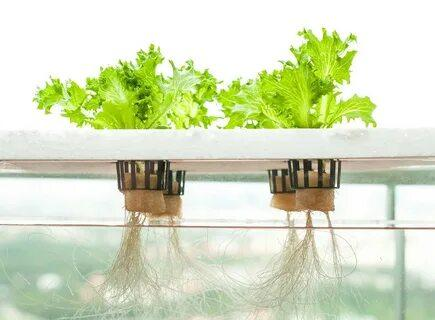
\includegraphics{images/hidrobonica.jpg}
    \caption{Метод выращивания --- гидропоника.}
    \label{fig:hidroponica}
\end{figure}

Гидропоника имеет ряд преимуществ перед традиционным выращиванием растений в почве, таких как:

\begin{enumerate}
    \item высокая производительность: растения получают оптимальное количество питательных веществ, которые идеально сбалансированы для их роста и развития;
    \item экономия воды: в гидропонике растения получают только ту воду, которая необходима для их жизни, что позволяет экономить до 90\% воды по сравнению с традиционным методом выращивания;
    \item экономия питательных веществ: раствор питательных веществ, используемый в гидропонике, может быть переработан и использован повторно, что позволяет экономить на затратах на удобрения;
    \item уменьшение риска заболеваний растений: гидропоника позволяет контролировать окружающую среду, что значительно уменьшает риск заражения растений различными заболеваниями;
    \item более быстрый рост растений: гидропоника позволяет растениям получать оптимальное количество питательных веществ, что способствует более быстрому росту и развитию.
\end{enumerate}

Недостатки гидропоники:

\begin{enumerate}
    \item высокие затраты на начальное оборудование и подготовку: для гидропоники требуется специальное оборудование и инфраструктура, что может стоить значительные средства;
    \item требуется постоянный контроль: гидропоника требует постоянного контроля и регулировки раствора питательных веществ, а также контроля за окружающей средой;
    \item зависимость от электричества: для работы гидропонической системы необходимо постоянное электропитание, что может быть проблематично в некоторых регионах.
\end{enumerate}

При использовании аэропоники корни растений обеспечиваются питательными растворами, которые распыляются на корни через форсунки или системы распыления. Это позволяет растениям получать необходимое количество кислорода и питательных веществ, что способствует их быстрому росту и развитию~\cite{Aeroponica}.

\begin{figure}[H]
    \centering
    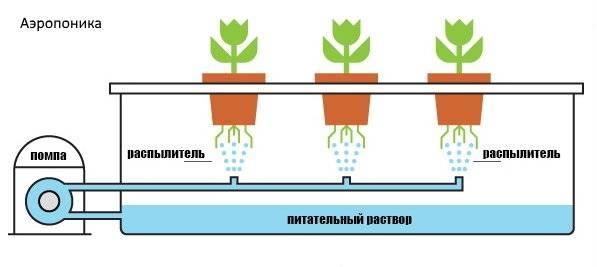
\includegraphics[scale=0.8]{images/aeroponica.jpg}
    \caption{Метод выращивания --- аэропоника.}
    \label{fig:aeroponica}
\end{figure}

Преимущества аэропоники:

\begin{enumerate}
    \item увеличение урожайности: в аэропонической системе растения получают более эффективный доступ к кислороду, питательным веществам и воде, что способствует более быстрому росту и высокой урожайности;
    \item экономия ресурсов: в аэропонической системе требуется меньше воды, чем при традиционном выращивании растений в почве, так как вода циркулирует в системе;
    \item устойчивость к болезням: растения в аэропонической системе меньше подвержены болезням, так как корневая система находится в воздухе, что предотвращает заражение растений грибковыми инфекциями и болезнями.
\end{enumerate}

Недостатки аэропоники:

\begin{enumerate}
    \item высокая стоимость установки: системы аэропоники требуют высокой точности и технологической сложности, что может привести к высокой стоимости установки;
    \item необходимость тщательного контроля: в аэропонической системе необходимо тщательно контролировать pH, уровень питательных веществ и кислорода, что требует дополнительного времени и усилий;
    \item высокая зависимость от электроэнергии: системы аэропоники требуют электричества для подачи питательных растворов, освещения и контроля климата.
\end{enumerate}

В системе аквапоники рыбы выступают как естественный источник питательных веществ для растений, а растения, в свою очередь, фильтруют воду и обеспечивают кислородом для рыб~\cite{Aquaponica}.

\begin{figure}[H]
    \centering
    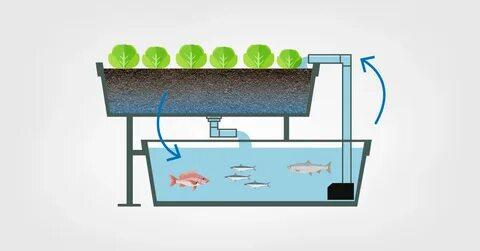
\includegraphics{images/aquaponica.jpg}
    \caption{Метод выращивания --- аквапоника.}
    \label{fig:aquaponica}
\end{figure}

Преимущества аквапоники:

\begin{enumerate}
    \item экологически чистое производство --- в аквапонике нет необходимости использовать химические удобрения и пестициды;
    \item экономия воды --- в аквапонике вода циркулирует и рециркулируется в системе, что позволяет значительно снизить расход воды по сравнению с традиционными методами выращивания растений;
    \item эффективное использование площади --- аквапоника позволяет получить высокие урожаи на относительно небольшой площади.
\end{enumerate}

Недостатки аквапоники:

\begin{enumerate}
    \item сложность технологии --- аквапоника требует точного баланса между питанием растений и уходом за рыбами, что может потребовать большого количества времени и усилий;
    \item высокие затраты на начальную установку системы --- установка системы аквапоники может требовать значительных инвестиций;
    \item низкая устойчивость системы --- неисправность одного из компонентов системы может повлиять на все остальные компоненты, что может привести к потере урожая.
\end{enumerate}

Вертикальное выращивание растений может использоваться в теплицах, зданиях и других сооружениях. Вертикальные теплицы могут иметь несколько ярусов, где на каждом ярусе находятся растения, поэтому этот метод выращивания может использоваться для получения высокой продуктивности на небольшой площади~\cite{Vertical}.

\begin{figure}[H]
    \centering
    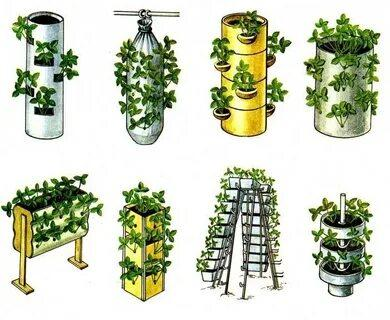
\includegraphics{images/vertical_growing.jpg}
    \caption{Вертикальное выращивание.}
    \label{fig:vertical_growing}
\end{figure}

Преимущества вертикального выращивания:

\begin{enumerate}
    \item увеличение урожайности: вертикальные теплицы позволяют выращивать больше растений на меньшей площади, что увеличивает урожайность;
    \item экономия пространства: вертикальное выращивание позволяет использовать вертикальное пространство, которое обычно не используется, поэтому этот метод особенно полезен для городских садов и огородов;
    \item контроль над условиями выращивания: в вертикальных теплицах можно контролировать освещение, температуру, влажность и другие условия выращивания, что позволяет получить оптимальные условия для роста и развития растений;
    \item меньше затрат на уход: вертикальные теплицы позволяют снизить затраты на уход за растениями, так как они могут быть автоматизированы.
\end{enumerate}

Недостатки вертикального выращивания:

\begin{enumerate}
    \item Большие затраты на оборудование: создание вертикальной теплицы может потребовать значительных затрат на оборудование и материалы;
    \item сложность управления условиями выращивания: управление условиями выращивания в вертикальных теплицах может быть сложным и требовать специальных знаний и навыков;
    \item ограниченность некоторых видов растений: некоторые растения могут быть трудно выращены в вертикальных теплицах из-за ограничений по доступу к свету и питательным веществам.
\end{enumerate}

Традиционное выращивание сельскохозяйственных культур было известно человечеству с древних времен и до сих пор является наиболее распространенным методом выращивания растительной продукции~\cite{Tradicional}.

\begin{figure}[H]
    \centering
    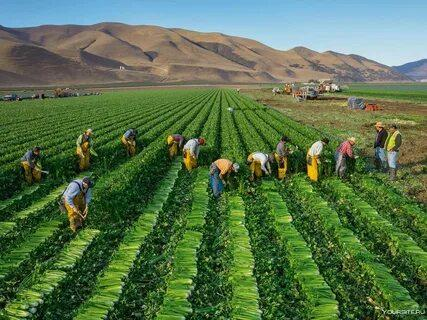
\includegraphics{images/tradicional_growing.jpg}
    \caption{Традиционное выращивание.}
    \label{fig:tradicional_growing}
\end{figure}

Преимущества традиционного выращивания:

\begin{enumerate}
    \item низкая стоимость. Выращивание на открытом грунте не требует крупных капиталовложений;
    \item естественный рост растений. Растения получают все необходимые для роста питательные вещества из почвы, что способствует их естественному развитию;
    \item широкий ассортимент продукции. В традиционном выращивании можно выращивать различные сорта овощей, фруктов и ягод, что позволяет получать разнообразную продукцию;
    \item устойчивость к изменениям погодных условий. В отличие от тепличного выращивания, традиционное выращивание не зависит от искусственного микроклимата.
\end{enumerate}

Недостатки традиционного выращивания:

\begin{enumerate}
    \item сезонность. В зависимости от региона, выращивание определенных культур возможно только в определенное время года;
    \item зависимость от погодных условий. Погода может негативно повлиять на урожайность и качество продукции;
    \item высокие затраты на уход. Ручной уход за посевами, полив и прочие меры заботы могут требовать значительных физических усилий;
    \item низкая урожайность. В сравнении с инновационными методами выращивания, традиционное выращивание не всегда обеспечивает высокую урожайность.
\end{enumerate}
